% =================================================================
%   Disposition --- IDC FSM & Datapath: BRZ (Branch on Zero)
%   62711 Digital Systems Design --- mundtlig eksamen
% =================================================================
\documentclass[11pt,a4paper]{article}

\usepackage[utf8]{inputenc}
\usepackage[T1]{fontenc}
\usepackage[english]{babel}
\usepackage[a4paper,margin=1.6cm]{geometry}
\usepackage{amsmath,amssymb}
\usepackage{xcolor}
\usepackage{tikz}
\usetikzlibrary{arrows.meta,positioning,calc}
\usepackage{enumitem}
\usepackage{microtype}

\setlist{itemsep=0.1em,topsep=0.1em,parsep=0pt}
\setlength{\parindent}{0pt}
\setlength{\parskip}{0.25em}

\definecolor{accent}{HTML}{1F4E79}
\definecolor{boxbg}{HTML}{F4F4F4}

% Tight section heading (replaces \section* to save vertical space)
\newcommand{\sect}[1]{\vspace{0.35em}\textcolor{accent}{\large\bfseries #1}\par\vspace{0.1em}}

% Stage direction (what to DO while speaking) --- visually distinct from spoken text
\newcommand{\gor}[1]{{\color{accent!90}\itshape$\rightarrow$\;\textbf{Gør:} #1}}

\begin{document}

{\centering\textcolor{accent}{\Large\bfseries Disposition --- IDC's FSM \& Datapath: \texttt{BRZ}}\par}
\vspace{0.5em}

% ======================== 1. Framing ============================
\sect{Hvad vi viser}
\begin{itemize}
  \item Vi sporer en \textbf{\texttt{BRZ}} (Branch on Zero) fra RAM $\to$ IR $\to$ IDC $\to$ PC.
  \item Hvorfor BRZ: \textbf{Mealy}-output ($=f$(state, IR, Z)) $\cdot$ \textbf{PS}-feltet (IDC's besked til PC) $\cdot$ \textbf{Z} er \textbf{kombinatorisk} (NOR af \emph{denne} cyklus' ALU).
\end{itemize}

% ======================== 2. FSM ================================
\sect{State machine --- BRZ bruger kun \textsc{inf} og \textsc{ex0}}

\begin{center}
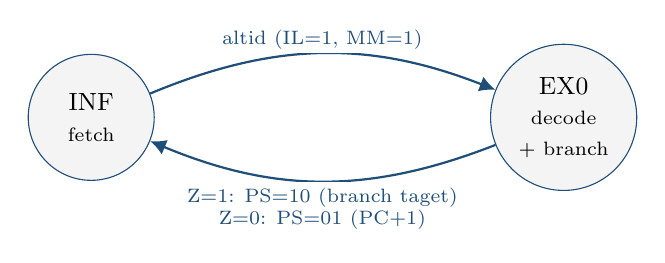
\begin{tikzpicture}[
  state/.style={
    draw=accent, fill=boxbg, circle,
    minimum size=16mm, align=center, font=\small
  },
  arr/.style={-{Latex[length=2mm,width=2mm]}, accent, thick}
]
  \node[state] (inf) at (0, 0) {INF\\\scriptsize fetch};
  \node[state] (ex0) at (6, 0) {EX0\\\scriptsize decode\\\scriptsize + branch};

  \draw[arr] (inf) to[bend left=22]
    node[above, font=\scriptsize, fill=white, inner sep=1pt]
    {altid (IL=1, MM=1)} (ex0);

  \draw[arr] (ex0) to[bend left=22]
    node[below, font=\scriptsize, align=center, fill=white, inner sep=2pt]
    {Z=1: PS=10 (branch taget)\\Z=0: PS=01 (PC+1)} (inf);
\end{tikzpicture}
\end{center}

\begin{itemize}
  \item Afkodningen sker kombinatorisk i EX0's \texttt{case IR(15 downto 9)}; \texttt{1100000} matcher BRZ-grenen.
\end{itemize}

% ======================== 3. Signalflow =========================
\sect{Signalflow gennem CPU'en}

\begin{center}
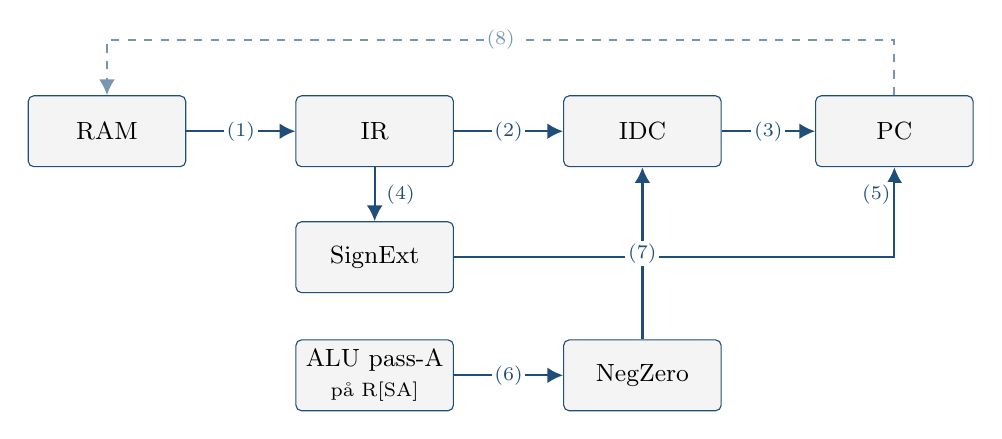
\begin{tikzpicture}[
  blk/.style={
    draw=accent, fill=boxbg, rounded corners=2pt,
    minimum height=9mm, minimum width=20mm,
    align=center, font=\small
  },
  arr/.style={-{Latex[length=2mm,width=2mm]}, accent, thick},
  lab/.style={font=\scriptsize, fill=white, inner sep=1pt}
]
  % Top row: RAM -> IR -> IDC -> PC
  \node[blk] (ram) at (0,    0)    {RAM};
  \node[blk] (ir)  at (3.4,  0)    {IR};
  \node[blk] (idc) at (6.8,  0)    {IDC};
  \node[blk] (pc)  at (10,   0)    {PC};

  % Sign Extender below IR + datapath Z-path
  \node[blk] (se)  at (3.4,  -1.6) {SignExt};
  \node[blk] (alu) at (3.4,  -3.1) {ALU pass-A\\\scriptsize på R[SA]};
  \node[blk] (nz)  at (6.8,  -3.1) {NegZero};

  \draw[arr] (ram.east) -- node[lab]{(1)} (ir.west);
  \draw[arr] (ir.east)  -- node[lab]{(2)} (idc.west);
  \draw[arr] (idc.east) -- node[lab]{(3)} (pc.west);
  \draw[arr] (ir.south) -- node[lab, right=1mm]{(4)} (se.north);
  \draw[arr] (se.east) -| node[lab, pos=0.85, left]{(5)} (pc.south);
  \draw[arr] (alu.east) -- node[lab]{(6)} (nz.west);
  \draw[arr] (nz.north) -- node[lab]{(7)} (idc.south);
  \draw[arr, dashed, accent!60]
    (pc.north) -- ++(0, 0.7) -| node[lab, pos=0.25]{(8)} (ram.north);
\end{tikzpicture}
\end{center}

\vspace{-0.3em}
{\footnotesize
\begin{center}
\begin{tabular}{@{}c l c l@{}}
\hline
\# & \textbf{Signal} & \textbf{Bredde} & \textbf{Rolle} \\
\hline
(1) & \texttt{Data\_Bus\_Out}     & 16b & instruktionsord fra RAM til IR \\
(2) & \texttt{IR(15:9)}           & 7b  & opcode til IDC \\
(3) & \texttt{PS}                 & 2b  & IDC's styring af PC (00/01/10/11) \\
(4) & \texttt{IR\{8,7,6,2,1,0\}}  & 6b  & rå offset-bits (Dx\,$\Vert$\,Bx) \\
(5) & \texttt{Offset}             & 8b  & sign-extended branch-offset til PC \\
(6) & \texttt{F}                  & 8b  & ALU-resultat (pass-A $=$ R[SA]) \\
(7) & \texttt{Z}                  & 1b  & NOR(F), zero-flag til IDC \\
(8) & \texttt{Address\_Out}       & 8b  & næste fetch-adresse (PC $\to$ RAM) \\
\hline
\end{tabular}
\end{center}
}

% ======================== 4. Kontrolord =========================
\sect{Kontrolord i de to cyklusser --- præcis hvad IDC sætter}

\textbf{Inputs IDC reagerer på (sensitivity list):} \texttt{current\_state}, \texttt{IR(15:9)=1100000}, \texttt{Z}.
\;(\texttt{N} kun for BRN; \texttt{V}, \texttt{C} ubrugt.)

\begin{center}
\small
\begin{tabular}{@{}l l l@{}}
\hline
\textbf{Output} & \textbf{INF (cyklus 0, fetch)} & \textbf{EX0 (cyklus 1, BRZ)} \\
\hline
\texttt{PS} & \texttt{00} (hold)        & \texttt{10} hvis Z=1 \ / \ \texttt{01} hvis Z=0 \\
\texttt{IL} & \texttt{1} (IR$\leftarrow$bus) & \texttt{0} \\
\texttt{MM} & \texttt{1} (PC$\to$adresse) & \texttt{0} \\
\texttt{RW} & \texttt{0}                & \texttt{0} \ (ingen registerskrivning) \\
\texttt{MW} & \texttt{0}                & \texttt{0} \\
\texttt{MD} & \texttt{0}                & \texttt{0} \\
\texttt{MB} & \texttt{0}                & \texttt{0} \\
\texttt{FS} & \texttt{0000}             & \texttt{0000} (pass-A) \\
\texttt{AX} & \texttt{0\&IR(5:3)}       & \texttt{0\&IR(5:3)} $=$ R[SA] \\
\texttt{DX} & \texttt{0\&IR(8:6)}       & \texttt{0\&IR(8:6)} (default) \\
\texttt{BX} & \texttt{0\&IR(2:0)}       & \texttt{0\&IR(2:0)} (default) \\
\hline
\end{tabular}
\end{center}

{\footnotesize\textit{Spec-tabel (PWB s.\,2): \texttt{FS}, \texttt{MB}, \texttt{MD} (+ top-bit) er don't-care \texttt{X} for BRZ; VHDL pinner dem til defaults ovenfor.}}

% (Pointe + Z-beslutning fjernet --- det siges i talepapiret; PS-værdierne står i FSM-diagrammet og tabellens PS-række)

% ======================== 5. Talepapir (egen side) ==============
% Tom side 2, så talepapiret havner på side 3.
% Duplex-print: ark 1 = reference (forside) + tom (bagside), ark 2 = talepapir
% --> reference og talepapir bliver to separate ark, der kan ligge ved siden af hinanden.
\newpage
\thispagestyle{empty}
\null
\newpage
\sect{Talepapir --- \texttt{BRZ} fra start til slut}

\textit{Normal tekst = det jeg siger.}\quad\gor{...} \textit{= det jeg gør imens (peger / skriver).}

\textbf{[Indledning]} Jeg præsenterer instruktionsafkoderen, IDC'en, og dens state machine ved at
følge instruktionen \texttt{BRZ} --- branch on zero --- fra hukommelsen og ud til program
counteren. BRZ viser tre ting på én gang: at IDC'en er en \emph{Mealy}-maskine, hvordan
\texttt{PS} styrer PC'en, og at zero-flaget er kombinatorisk.

BRZ er i bund og grund en \emph{if-sætning} i hardware. Eksempel: i et LED-show hvor vi slukker
dioderne, kan vi teste LED-mønstret med BRZ --- når alle bits er nul (alle LED'er slukket),
brancher vi hen til det vi vil gøre bagefter. Uden en betinget branch kunne programmet kun køre
lige ud.

\gor{skriv på tavlen} \quad\texttt{BRZ\ \ \ Dx\ \ \ Ax\ \ \ Bx}

BRZ har tre felter. \texttt{Ax} er det register vi tester --- det skal være nul for at vi
brancher. \texttt{Dx} og \texttt{Bx} er \emph{tilsammen} offsettet, altså hvor langt vi hopper.
Jeg viser om lidt hvordan de to limes sammen.

\textbf{[Overblik]} CPU'en er en datapath plus en mikroprogram-controller. IDC'en sidder i
controlleren og udsender et 28-bit kontrolord hver klokcyklus --- værdierne står i tabellen på
forrige side. BRZ tager to cyklusser og bruger kun \textsc{inf} og \textsc{ex0}.
\gor{peg på state machine-diagrammet: \textsc{inf} $\to$ \textsc{ex0} $\to$ \textsc{inf}.}

\textbf{[Cyklus 0 --- \textsc{inf}, fetch]} Først henter vi instruktionen. IDC'en sætter
\texttt{IL=1} og \texttt{MM=1}; \texttt{MM=1} gør at PC'en driver adressen ud til RAM'en, ordet
kommer tilbage ad \texttt{Data\_Bus\_Out}, og \texttt{IL=1} loader det ind i IR på næste
klokflanke.
\gor{før fingeren langs signalet: PC $\to$ MUX M $\to$ RAM $\to$ MUX MR $\to$ IR.}

\textbf{[Cyklus 1 --- \textsc{ex0}, decode]} Nu afkoder IDC'en opcoden \texttt{IR(15:9)} i et
\texttt{case}-statement; \texttt{1100000} er BRZ.
\gor{peg IR $\to$ IDC.}

\textbf{[Z dannes parallelt]} Samtidig står alle andre signaler på default. Default'en sætter
\texttt{AX} til R[SA] --- altså \texttt{Ax}-feltet --- og \texttt{FS=0000}, som er pass-A. R[SA]
løber uændret gennem ALU'en, og NegZero regner \texttt{Z} ud kombinatorisk: \texttt{Z=1} kun hvis
R[SA] er nul. \texttt{RW=0}, så intet register skrives.
\gor{før fingeren: R[SA] $\to$ ALU (pass-A) $\to$ NegZero $\to$ \texttt{Z} $\to$ IDC.}

\textbf{[Tilbage ved IR --- sign extenderen]} Så tilbage til IR for offsettet. Sign Extenderen
tager netop \texttt{Dx} og \texttt{Bx}, limer dem sammen til et 6-bit tal --- \texttt{Dx} først,
så \texttt{Bx} --- og sign-extender til de 8 bit PC'en forventer.
\gor{før fingeren IR $\to$ SignExt $\to$ PC, og skriv på tavlen:}
\[
  \texttt{Dx}=\texttt{101},\ \ \texttt{Bx}=\texttt{010}
  \ \ \Rightarrow\ \ \texttt{101010}\ (6\,\text{bit})
  \ \ \xrightarrow{\ \text{sign-ext}\ }\ \ \texttt{11101010}\ (8\,\text{bit}) \;=\; -22
\]
Det øverste bit i \texttt{Dx} --- her \texttt{1} --- er fortegnet; det kopieres op i de nye høje
bits, så værdien beholder sit fortegn. Her er offsettet negativt, så vi hopper baglæns.
Det færdige 8-bit offset føres til PC'ens adder og lægges til den nuværende PC ---
\(PC \leftarrow PC + \text{offset}\) --- så med $-22$ hopper vi 22 pladser tilbage.

\textbf{[Beslutningen --- Mealy]} Og her er Mealy-pointen: outputtet afhænger af \texttt{Z} her og
nu. Er \texttt{Z=1} sætter IDC'en \texttt{PS=10}, additionen ovenfor sker, og branchen tages. Er
\texttt{Z=0} sætter den \texttt{PS=01}, og PC'en springer additionen over og tæller bare én op
($PC+1$).
\gor{før fingeren IDC $\to$ \texttt{PS} $\to$ PC.}

\textbf{[Perspektiv --- BRZ vs JMP]} Til sammenligning er JMP \emph{ubetinget} og \emph{absolut}.
BRZ er betinget (kun hvis \texttt{Z=1}) og \emph{relativ} --- $PC \leftarrow PC + \text{offset}$,
\texttt{PS=10}. JMP sætter i stedet \texttt{PS=11} og loader hele adressen direkte fra et
register: $PC \leftarrow R[SA]$ (Address\_In). JMP bruger altså \emph{hverken} Sign Extenderen
eller additionen, og kan ramme hele adresserummet --- mens BRZ kun når $-32\ldots+31$ omkring
den nuværende PC.
\gor{skriv på tavlen:}\quad BRZ: $PC\!\leftarrow\!PC+\text{offset}$ (\texttt{PS=10}) \quad vs \quad JMP: $PC\!\leftarrow\!R[SA]$ (\texttt{PS=11})

\textbf{[Afrunding]} Begge veje vender tilbage til \textsc{inf} --- to cyklusser i alt. Tre
pointer: \texttt{PS} er hele interfacet mellem IDC og PC; \texttt{Z} er kombinatorisk, så vi
tester R[SA] lige nu; og \texttt{BRN} er identisk på nær opcode og flag. Det var \texttt{BRZ} fra
start til slut. Tak.

\end{document}
